% =============================================================================
%  Chapter 2 — Cơ sở lý thuyết & Các công trình liên quan
% =============================================================================
%  Cấu trúc:
%    chapter02/
%      ├── 01_intro.tex             — Mở đầu chương
%      ├── 02_cheo_features.tex     — 2.1  Các đặc tính của nghệ thuật Chèo
%      ├── 03_knowledge_repr.tex    — 2.2  Các hình thức biểu diễn tri thức
%      ├── 04_rag_systems.tex       — 2.3  Các hệ thống sinh tăng cường truy hồi
%      ├── 05_related_works.tex     — 2.4  Các công trình liên quan
%      └── 06_summary.tex           — Tiểu kết
% =============================================================================

% =============================================================================
%  Chapter 2 — Cơ sở lý thuyết & Các công trình liên quan
%  Section: Mở đầu chương
% =============================================================================

Chương này trình bày các cơ sở lý thuyết nền tảng phục vụ cho đề tài, bao gồm các phương pháp biểu diễn tri thức có cấu trúc như Ontology và Knowledge Graph, cùng với các kiến trúc truy hồi – tạo sinh hiện đại như Retrieval-Augmented Generation (RAG) và GraphRAG. Các khái niệm này đóng vai trò quan trọng trong việc tổ chức, khai thác và suy luận tri thức, đồng thời là nền tảng cho hệ thống được đề xuất trong khóa luận. Bên cạnh đó, chương cũng tổng hợp và phân tích các công trình nghiên cứu liên quan nhằm làm rõ bối cảnh và định hướng nghiên cứu.

% =============================================================================
%  Section 2.1 — Các đặc tính của nghệ thuật Chèo
% =============================================================================

\section{Các đặc tính của nghệ thuật Chèo}

Chèo là một loại hình sân khấu dân gian truyền thống của Việt Nam, mang tính tự sự cao và phản ánh đời sống xã hội thông qua hình thức diễn xướng tổng hợp. Tuy nhiên, trong phạm vi nghiên cứu này, điều quan trọng không chỉ nằm ở giá trị văn hóa của chèo, mà ở các đặc trưng cấu trúc và biểu đạt của nó – những yếu tố trực tiếp chi phối cách thức mô hình hóa tri thức dưới dạng bản thể luận (Ontology) và Knowledge Graph.

Trước hết, đặc trưng nổi bật nhất của chèo là cấu trúc tự sự phân lớp. Một vở chèo không được tổ chức theo chuỗi hồi – cảnh với quan hệ nhân quả chặt chẽ như kịch phương Tây, mà bao gồm nhiều lớp diễn tương đối độc lập về nội dung. Mỗi lớp diễn thường tập trung vào một tình huống, một xung đột hoặc một khía cạnh tính cách nhân vật cụ thể. Điều này tạo ra một cấu trúc dạng mô-đun, trong đó các lớp diễn có thể được xem như các đơn vị tri thức riêng biệt, vừa có tính độc lập tương đối, vừa có thể liên kết với nhau thông qua cốt truyện tổng thể. Chính đặc điểm này đặc biệt phù hợp với việc biểu diễn tri thức dưới dạng đồ thị, nơi mỗi lớp diễn có thể được mô hình hóa như một thực thể (entity) hoặc một nút (node), và các mối quan hệ giữa chúng được biểu diễn dưới dạng các cạnh (edges).

Thứ hai, hệ thống nhân vật trong chèo mang tính tượng hình và có cấu trúc phân loại rõ ràng. Các mô hình nhân vật như Đào, Kép, Hề, Lão và Mụ không chỉ đóng vai trò là các nguyên mẫu (archetype) trong nghệ thuật biểu diễn, mà còn tạo ra một hệ phân cấp (hierarchy) tự nhiên, rất thuận lợi cho việc xây dựng các lớp (class) trong Ontology. Từ các mô hình cơ bản này, có thể phát triển các tiểu loại chi tiết hơn dựa trên đặc điểm tính cách, vai trò trong cốt truyện hoặc vị thế xã hội. Điều đó cho thấy hệ thống nhân vật chèo không chỉ giàu tính biểu đạt mà còn có cấu trúc phân loại rõ ràng, phù hợp với các phương pháp biểu diễn tri thức dựa trên phân cấp và kế thừa.

Thứ ba, mối quan hệ giữa các thành phần trong chèo mang tính ngữ nghĩa phong phú và đa dạng. Các quan hệ như “nhân vật tham gia lớp diễn”, “lớp diễn thuộc vở diễn”, hay “nhân vật đối lập/ hỗ trợ lẫn nhau” đều có thể được xác định một cách rõ ràng và nhất quán. Đây là cơ sở quan trọng để xây dựng các quan hệ (relations) trong Knowledge Graph, cho phép thực hiện các truy vấn phức tạp và suy luận ngữ nghĩa. Đặc biệt, do mỗi lớp diễn thường làm nổi bật một khía cạnh cụ thể của nhân vật, nên mối quan hệ giữa nhân vật và lớp diễn có thể được khai thác để biểu diễn sự phát triển hoặc biến đổi của nhân vật trong toàn bộ vở chèo.

Thứ tư, nội dung của chèo thường dựa trên các mô-típ quen thuộc của văn học dân gian, với hệ thống giá trị đạo đức được thể hiện tương đối rõ ràng. Điều này giúp việc trích xuất và chuẩn hóa tri thức trở nên thuận lợi hơn, do các khái niệm và quan hệ thường mang tính ổn định và có thể được định nghĩa một cách nhất quán. Đồng thời, sự xuất hiện của các nhân vật có tính chất trung gian hoặc phức tạp về tâm lý trong một số vở chèo cũng mở ra khả năng biểu diễn các quan hệ ngữ nghĩa tinh vi hơn, chẳng hạn như các mức độ mâu thuẫn nội tâm hoặc chuyển biến tâm lý.

Từ các đặc trưng trên, có thể thấy rằng nghệ thuật chèo sở hữu một cấu trúc tri thức tự nhiên phù hợp với việc mô hình hóa dưới dạng Ontology và Knowledge Graph. Do đó, trong khóa luận này, hệ thống Ontology được thiết kế theo hướng phân tầng, bao gồm các lớp chính như vở diễn, lớp diễn và nhân vật, cùng với các quan hệ ngữ nghĩa tương ứng. Cách tiếp cận này không chỉ phản ánh trung thực đặc trưng của chèo, mà còn tạo nền tảng cho việc xây dựng hệ thống GraphRAG có khả năng truy vấn và suy luận hiệu quả trên dữ liệu văn hóa phi cấu trúc.

% =============================================================================
%  Section 2.2 — Các hình thức biểu diễn tri thức
% =============================================================================

\section{Các hình thức biểu diễn tri thức}

Trong các hệ thống trí tuệ nhân tạo hiện đại, đặc biệt là các hệ thống khai thác tri thức có cấu trúc, Ontology và đồ thị tri thức giữ vai trò nền tảng trong việc tổ chức, chuẩn hóa và biểu diễn thông tin. Dữ liệu văn bản thuần túy chỉ phản ánh tri thức ở dạng phi cấu trúc, trong khi đó Ontology và đồ thị tri thức cho phép mô hình hóa rõ ràng các khái niệm, thực thể và quan hệ giữa chúng. Điều này có ý nghĩa lớn với các miền tri thức có cấu trúc quan hệ phức tạp như nghệ thuật Chèo, nơi tồn tại sự liên kết đa tầng giữa nhân vật, vở diễn, vai diễn, làn điệu, bối cảnh lịch sử, ... Phần này trình bày cơ sở lý thuyết của bản thể luận và đồ thị tri thức, đồng thời làm rõ vai trò của chúng trong việc xây dựng hệ thống truy xuất tri thức có cấu trúc.

\subsection{Bản thể luận - Ontology}

Ontology là một mô hình hình thức hóa tri thức của một miền xác định, trong đó các khái niệm và quan hệ giữa chúng được định nghĩa một cách tường minh và có cấu trúc. Trong khoa học máy tính, ontology là một hệ thống bao gồm các lớp khái niệm (classes), thuộc tính (properties) và các ràng buộc logic nhằm đảm bảo tính nhất quán ngữ nghĩa. Việc hình thức hóa này cho phép các mô hình ngôn ngữ lớn hiểu được cấu trúc của miền tri thức, thay vì chỉ xử lý dữ liệu ở mức ký hiệu hoặc chuỗi văn bản. Nhờ đó, ontology tạo tiền đề cho các cơ chế suy luận tự động và chuẩn hóa kho thông tin.

Cấu trúc của một ontology thường được tổ chức theo phân cấp khái niệm, trong đó các lớp có thể kế thừa thuộc tính và quan hệ từ lớp cha. Các thuộc tính được chia thành thuộc tính đối tượng (object properties), mô tả quan hệ giữa các thực thể, và thuộc tính dữ liệu (data properties), mô tả giá trị cụ thể của thực thể. Trong miền nghệ thuật Chèo, ontology có thể xác định rõ ràng mối quan hệ giữa các khái niệm như vở diễn, nhân vật, vai diễn và nghệ sĩ, từ đó tạo ra một khung khái niệm thống nhất cho toàn bộ hệ thống.

Về mặt kỹ thuật, ontology thường được biểu diễn bằng các chuẩn như Resource Description Framework (RDF), Resource Description Framework Schema (RDFS) và Web Ontology Language (OWL), trong đó OWL hỗ trợ biểu diễn các ràng buộc logic phức tạp và tích hợp với các bộ suy luận tự động. Trong các hệ thống biểu diễn tri thức hiện đại, ontology thường đóng vai trò như một tầng lược đồ khái niệm (schema layer), định nghĩa cấu trúc và ngữ nghĩa của miền tri thức. Dựa trên lược đồ này, các thực thể và quan hệ cụ thể có thể được tổ chức thành một đồ thị tri thức, cho phép lưu trữ và khai thác dữ liệu ở quy mô lớn.

\subsection{Đồ thị tri thức - Knowledge Graph}

Đồ thị tri thức là một mô hình biểu diễn tri thức dưới dạng đồ thị, trong đó các thực thể được biểu diễn bởi các nút (nodes) và các quan hệ giữa chúng được biểu diễn bởi các cạnh (edges). Mỗi đơn vị tri thức thường được mô tả dưới dạng bộ ba \textit{(subject – predicate – object)}, cho phép biểu diễn thông tin một cách linh hoạt, trực quan và dễ mở rộng. Khác với các mô hình cơ sở dữ liệu truyền thống vốn phụ thuộc vào cấu trúc bảng cố định, đồ thị tri thức cho phép bổ sung thực thể và quan hệ mới mà không làm thay đổi lược đồ tổng thể, từ đó phù hợp với các miền tri thức có tính mở và liên tục phát triển.

Trong hệ thống biểu diễn tri thức hiện đại, đồ thị tri thức được xây dựng dựa trên nền tảng Ontology. Ontology đóng vai trò là tầng khái niệm (schema layer), định nghĩa các lớp, thuộc tính và ràng buộc logic của miền tri thức, còn đồ thị tri thức là tầng dữ liệu (instance layer), trong đó các thực thể cụ thể và các mối quan hệ giữa chúng được hiện thực hóa theo cấu trúc đã được quy định. Sự phân tách này giúp đảm bảo rằng dữ liệu trong đồ thị tri thức được tổ chức một cách có hệ thống, đồng thời tuân thủ các ràng buộc ngữ nghĩa, từ đó hỗ trợ khả năng suy luận và kiểm tra tính nhất quán.

Về mặt triển khai, đồ thị tri thức có thể được xây dựng theo hai hướng tiếp cận chính. Thứ nhất là mô hình RDF triple store, trong đó dữ liệu được lưu trữ dưới dạng các bộ ba và phù hợp với các hệ thống chú trọng suy luận ngữ nghĩa dựa trên các chuẩn như RDF, RDFS và OWL. Thứ hai là mô hình property graph, được sử dụng trong các hệ quản trị cơ sở dữ liệu đồ thị như Neo4j, cho phép gán thuộc tính trực tiếp lên các nút và cạnh, từ đó hỗ trợ hiệu quả các truy vấn theo đường đi và truy vấn đa bước. Việc lựa chọn mô hình phụ thuộc vào yêu cầu cụ thể của hệ thống, bao gồm khả năng suy luận, hiệu năng truy vấn và tính linh hoạt trong mở rộng dữ liệu.

Đồ thị tri thức có khả năng biểu diễn các quan hệ đa chiều và phức tạp mà không làm gia tăng độ phức tạp của lược đồ. Đồ thị tri thức không cần thực hiện các phép nối (join) phức tạp như trong cơ sở dữ liệu quan hệ, các truy vấn trên đồ thị tri thức có thể khai thác trực tiếp cấu trúc liên kết giữa các thực thể thông qua các đường đi trong đồ thị. Điều này đặc biệt hữu ích trong các bài toán yêu cầu khám phá tri thức hoặc truy vấn theo ngữ cảnh, nơi mà các mối quan hệ giữa dữ liệu đóng vai trò quan trọng. Ngoài ra, đồ thị tri thức còn đóng vai trò quan trọng trong việc nâng cao khả năng giải thích của hệ thống. Mỗi kết quả truy vấn không chỉ là một giá trị đầu ra, mà còn có thể được truy vết thông qua chuỗi các quan hệ cụ thể giữa các thực thể trong đồ thị. Điều này giúp tăng tính minh bạch và độ tin cậy, đặc biệt trong các hệ thống hỏi đáp yêu cầu khả năng giải thích quyết định.

Trong bối cảnh các hệ thống truy hồi tri thức hiện đại, đặc biệt là Retrieval-Augmented Generation (RAG), đồ thị tri thức được sử dụng như một nguồn tri thức có cấu trúc nhằm hỗ trợ quá trình truy vấn và mở rộng ngữ cảnh \cite{fan2023cichmkg,wan2024wumkg}. Khi được kết hợp với Ontology, đồ thị tri thức không chỉ cung cấp dữ liệu mà còn kế thừa các ràng buộc ngữ nghĩa của miền tri thức, từ đó nâng cao chất lượng truy hồi và hỗ trợ các cơ chế suy luận. Trong phạm vi nghiên cứu này, đồ thị tri thức đóng vai trò là lớp lưu trữ và khai thác dữ liệu, được xây dựng dựa trên Ontology nhằm đảm bảo tính nhất quán và phục vụ các thành phần khác của hệ thống.

% =============================================================================
%  Section 2.3 — Các hệ thống sinh tăng cường truy hồi
% =============================================================================

\section{Các hệ thống sinh tăng cường truy hồi }
\subsection{Phương pháp tạo sinh tăng cường truy hồi truyền thống - RAG}

Retrieval-Augmented Generation (RAG) \cite{lewis2020rag} là kiến trúc kết hợp giữa mô hình truy hồi thông tin và mô hình sinh ngôn ngữ nhằm nâng cao độ chính xác của câu trả lời. Thay vì để mô hình ngôn ngữ sinh nội dung hoàn toàn dựa trên tập dữ liệu mà nó được huấn luyện, hệ thống RAG thực hiện truy vấn từ một kho dữ liệu bên ngoài để tìm các đoạn văn bản liên quan đến câu hỏi. Các đoạn văn bản này sau đó được đưa vào prompt làm ngữ cảnh bổ sung, từ đó giúp mô hình đưa ra câu trả lời dựa trên thông tin cụ thể hơn. Cách tiếp cận này cho phép hệ thống khai thác hệ thống tri thức được cập nhật liên tục và giảm nguy cơ tạo ra nội dung sai lệch.

Trong kiến trúc RAG truyền thống (Hình \ref{fig:overviewRAG}), quy trình thường bao gồm các bước: mã hóa câu hỏi thành dạng vector, tìm kiếm các đoạn văn bản có độ tương đồng cao trong cơ sở dữ liệu vector (tương đồng về mặt ngữ nghĩa), và kết hợp các đoạn này vào prompt trước khi gửi đến mô hình ngôn ngữ. Phương pháp này có ưu điểm là không yêu cầu huấn luyện lại mô hình và có thể dễ dàng tích hợp với các cơ sở dữ liệu mới. Tuy nhiên, RAG truyền thống chủ yếu dựa trên độ tương đồng ngữ nghĩa giữa các đoạn văn bản, do đó việc truy hồi phụ thuộc mạnh vào chiến lược chia nhỏ văn bản (chunking) và chất lượng mã hóa (embedding).

\begin{figure}
    \centering
    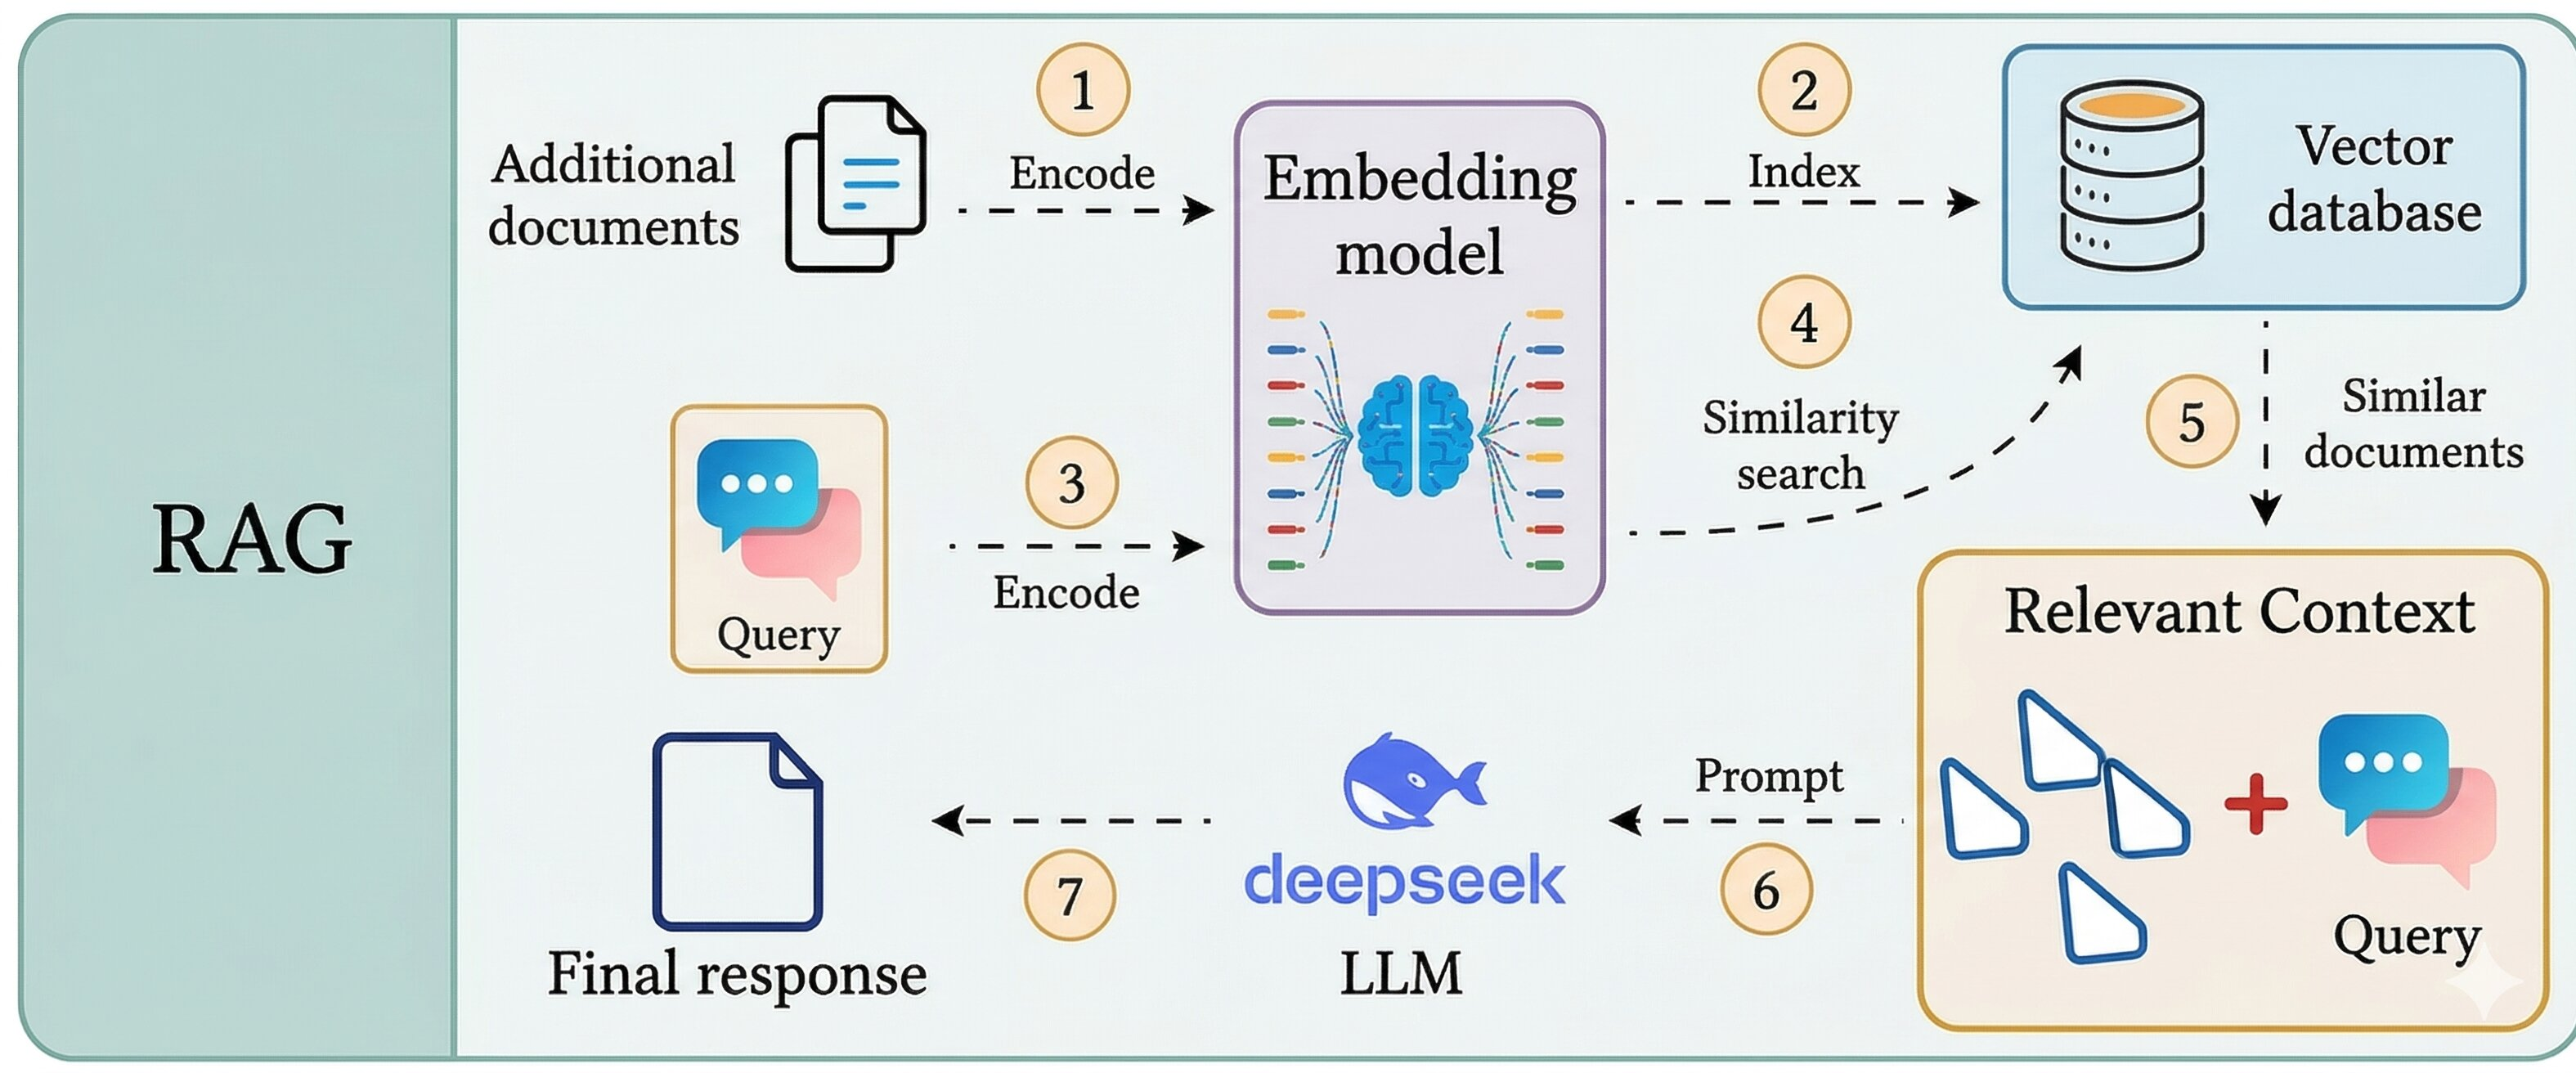
\includegraphics[width=0.9\linewidth]{figures//c2/RAG.jpg}
    \caption{Tổng quan kiến trúc RAG}
    \label{fig:overviewRAG}
\end{figure}

Một hạn chế cốt lõi của RAG truyền thống là thiếu khả năng khai thác cấu trúc quan hệ giữa các thực thể. Khi câu hỏi yêu cầu tổng hợp thông tin từ nhiều nguồn hoặc yêu cầu suy luận đa bước, việc chỉ truy hồi các đoạn văn bản rời rạc có thể không cung cấp đủ ngữ cảnh cần thiết. Ngoài ra, RAG khó đảm bảo rằng các đoạn văn bản được truy hồi có mối liên hệ logic chặt chẽ với nhau, bởi cơ chế truy hồi chủ yếu dựa trên mức tương đồng ngữ nghĩa. Chính những hạn chế này đã thúc đẩy sự phát triển của các phương pháp tích hợp tri thức có cấu trúc hơn, trong đó GraphRAG là một hướng tiếp cận tiêu biểu.

\subsection{Phương pháp tạo sinh tăng cường truy hồi dựa trên đồ thị - GraphRAG}

GraphRAG \cite{gong2025triplet,zhu2025kgguidedrag,hu2025grag} là một mở rộng của kiến trúc RAG, thay vì làm việc với cơ sở dữ liệu với hàng triệu bản ghi dạng chữ, dạng bảng thì nó làm việc với cơ sở tri thức là đồ thị tri thức. Trong đó tầng truy hồi thông tin không chỉ dựa trên độ tương đồng ngữ nghĩa mà còn khai thác cấu trúc quan hệ đang tồn tại của đồ thị tri thức. Thay vì truy hồi các đoạn văn bản độc lập, hệ thống có thể truy xuất các thực thể và quan hệ liên quan trong đồ thị tri thức (Hình \ref{fig:overview_graphrag}), từ đó xây dựng mạng lưới thông tin phù hợp với truy vấn. Mạng lưới thông tin này sau đó được chuyển đổi thành dạng ngữ cảnh văn bản hoặc biểu diễn có cấu trúc để cung cấp cho mô hình ngôn ngữ. Nhờ đó, quá trình sinh câu trả lời được định hướng bởi cấu trúc quan hệ thay vì chỉ dựa vào độ tương đồng ngữ nghĩa thông qua mã hóa thông tin.

\begin{figure}
    \centering
    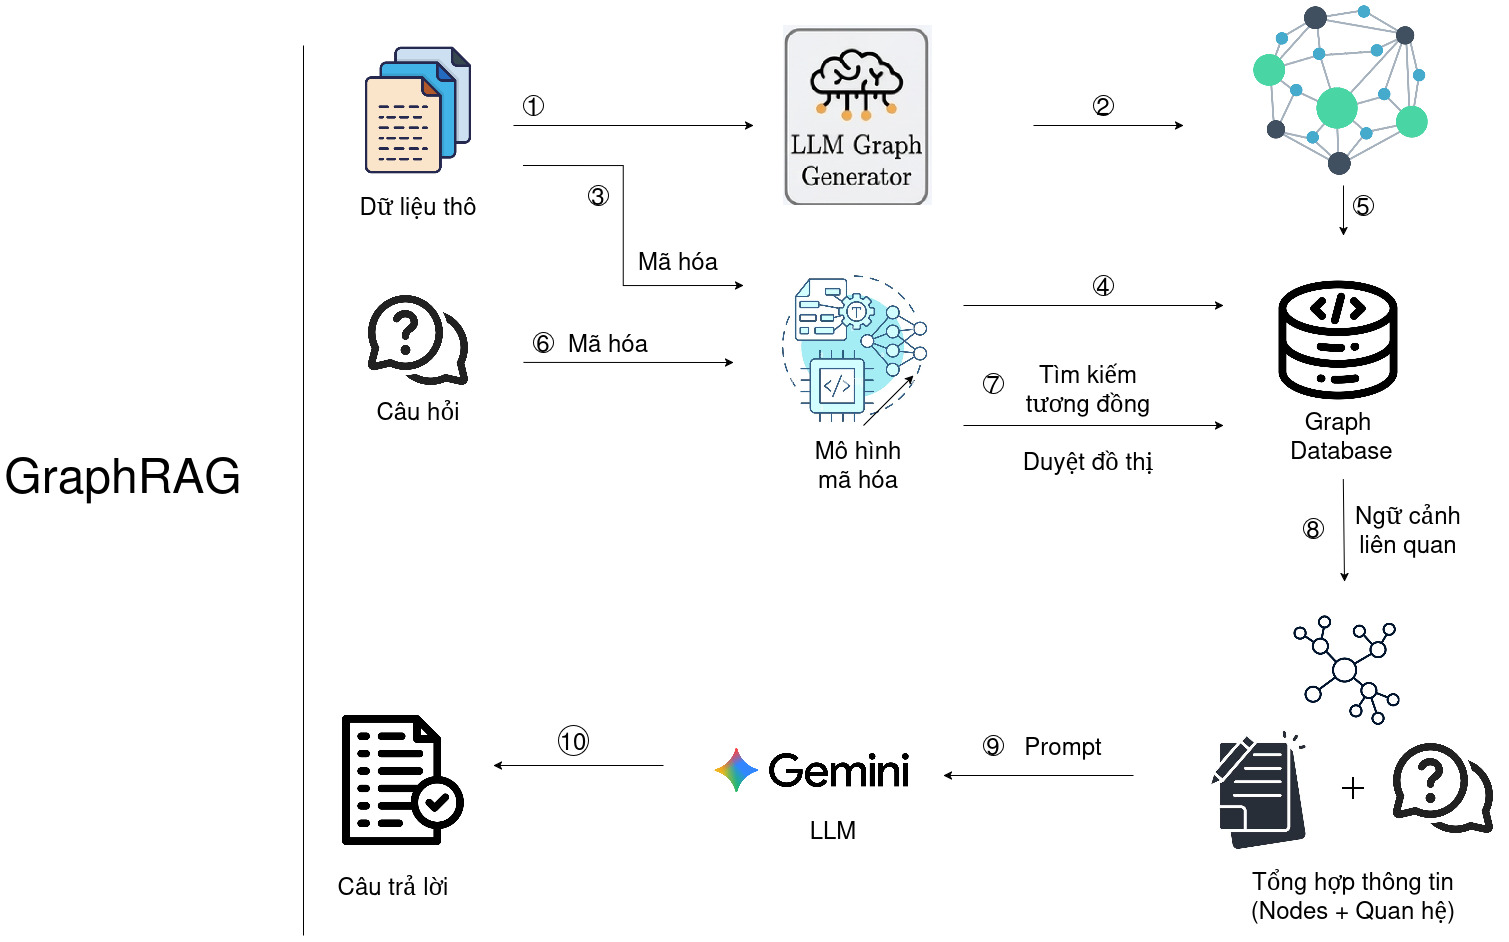
\includegraphics[width=0.9\linewidth]{figures//c2/GraphRAG.jpg}
    \caption{Tổng quan kiến trúc GraphRAG}
    \label{fig:overview_graphrag}
\end{figure}

Điểm khác biệt quan trọng giữa RAG truyền thống và GraphRAG nằm ở khả năng hỗ trợ suy luận đa bước. Trong khi RAG chủ yếu truy hồi các đoạn văn bản có liên quan trực tiếp đến câu hỏi, GraphRAG có thể mở rộng truy vấn thông qua các cạnh trong đồ thị để khám phá các thực thể liên quan gián tiếp. Với khả năng này, GraphRAG có thể trả lời được các câu hỏi yêu cầu tổng hợp thông tin từ nhiều nguồn hoặc yêu cầu phân tích mối quan hệ giữa các thực thể. Đồ thị tri thức được xây dựng kĩ lưỡng sẽ giúp đảm bảo rằng ngữ cảnh được cung cấp cho mô hình có tính liên kết logic, thay vì là tập hợp các đoạn văn bản rời rạc. Đồng thời, các câu trả lời của GraphRAG có mức tin cậy cao nhờ việc xây dựng từng đồ thị con với từng câu hỏi, mỗi câu trả lời có thể được truy vết thông qua chuỗi quan hệ giữa các thực thể trong đồ thị tri thức.

Trong phạm vi nghiên cứu này, GraphRAG được sử dụng như một cơ chế tổ chức và cung cấp tri thức có cấu trúc cho hệ thống trả lời câu hỏi. Mô hình ngôn ngữ đóng vai trò thành phần sinh câu trả lời, trong khi đồ thị tri thức đảm nhiệm việc điều hướng và mở rộng ngữ cảnh dựa trên quan hệ thực thể. Sự kết hợp này cho phép tận dụng khả năng sinh ngôn ngữ của mô hình đồng thời khai thác cấu trúc tri thức của đồ thị.

% =============================================================================
%  Section 2.4 — Các công trình liên quan
% =============================================================================

\section{Các công trình liên quan}

Để giải quyết bài toán biểu diễn và truy vấn tri thức, nhiều hướng tiếp cận đã được đề xuất trong những năm gần đây. Dựa trên đặc thù kỹ thuật và phương pháp tích hợp tri thức, các nghiên cứu đi trước có thể được phân loại thành ba nhóm chính. Các nhóm này đều đạt được các cột mốc đáng kể trong việc hỗ trợ giảm sự mơ hồ trong tri thức của LLMs tuy nhiên mỗi nhóm đều bộc lộ những hạn chế cụ thể khi áp dụng vào miền tri thức nghệ thuật có cấu trúc phức tạp như nghệ thuật Chèo.

Nhóm nghiên cứu đầu tiên tập trung vào các hệ thống hỏi đáp dựa trên đồ thị tri thức (KGQA) và ứng dụng đồ thị tri thức (KG) trong biểu diễn di sản văn hóa. Các công trình của Fan et al. \cite{fan2023cichmkg}, Wan et al. \cite{wan2024wumkg} và Huang et al. \cite{huang2023using} đã khẳng định khả năng ưu việt của KG trong việc kết nối các nguồn dữ liệu văn hóa phân mảnh. Tuy nhiên, hạn chế cốt lõi của các dự án này là mới dừng lại ở khâu tổ chức và lưu trữ dữ liệu, thiếu sự tích hợp với các mô hình sinh ngôn ngữ tự nhiên để tạo thành một hệ thống hỏi đáp hoàn chỉnh. Mặt khác, đối với các hệ thống KGQA truyền thống, các nghiên cứu dựa trên semantic parsing như Sun et al. (2020)\cite{sun2020sparqa} và Yin et al. (2016) \cite{yih2015semantic} đã chỉ ra rằng phương pháp này phụ thuộc mạnh vào việc phân tích cú pháp và các mẫu truy vấn được định nghĩa sẵn. Sự phụ thuộc này khiến hệ thống trở nên kém linh hoạt và gặp khó khăn khi xử lý các truy vấn phức tạp hoặc yêu cầu suy luận đa bước.

Nhóm nghiên cứu thứ hai liên quan đến kiến trúc Retrieval-Augmented Generation (RAG) do Lewis et al. \cite{lewis2020retrieval} khởi xướng. Phương pháp này giải quyết được bài toán cập nhật tri thức cho LLMs mà không cần huấn luyện lại. Mặc dù vậy, RAG truyền thống tồn tại nhược điểm lớn về "truy xuất phẳng". Bằng cách chia nhỏ tài liệu thành các đoạn văn bản độc lập và so khớp dựa trên độ tương đồng vector (embedding), cơ chế này vô tình cắt đứt cấu trúc quan hệ nội tại giữa các thực thể. Do đó, đối với các truy vấn yêu cầu tổng hợp thông tin từ nhiều nguồn hoặc theo dấu các liên kết logic phức tạp, RAG thường thất bại trong việc cung cấp một ngữ cảnh đủ sâu và liền mạch.

Nhóm nghiên cứu thứ ba tập trung vào kiến trúc Graph-based RAG (GraphRAG), ra đời nhằm khắc phục hạn chế của RAG bằng cách tích hợp trực tiếp cấu trúc đồ thị vào quá trình truy xuất. Các công trình như KG-guided RAG \cite{zhu2025knowledge} hay GRAG \cite{hu2025grag} đã sử dụng KG để định hướng việc mở rộng ngữ cảnh một cách hiệu quả. Tiến xa hơn, các hệ thống SG-RAG \cite{saleh2025sgrag} và KRAGEN \cite{matsumoto2024kragen} tập trung truy xuất các tiểu đồ thị (subgraph), trong khi phương pháp của Gong et al. \cite{gong2025beyond} khai thác sâu bộ ba quan hệ (triplet-driven). Hiện tại, các hệ thống GraphRAG hiện hành vẫn vấp phải một rào cản kỹ thuật lớn: chúng bị giới hạn ở cơ chế truy xuất đơn độ hạt (single-granularity). Việc cố định một mức độ truy xuất làm hệ thống thiếu tính linh hoạt khi phải xử lý đa dạng các loại câu hỏi, từ định danh thực thể cục bộ đến phân tích toàn cục. Thêm vào đó, các kiến trúc này chủ yếu được phát triển cho các miền tri thức phổ quát hoặc y sinh. Khi áp dụng vào nghệ thuật sân khấu dân gian—nơi hệ thống nhân vật và lớp diễn có sự biến thiên liên tục—chúng bộc lộ sự thiếu tương thích trầm trọng do thiếu một Ontology chuyên biệt.

Từ những khoảng trống nghiên cứu và hạn chế kỹ thuật của các công trình đi trước, sự cần thiết của một hệ thống tối ưu hóa riêng cho nghệ thuật Chèo trở nên vô cùng rõ ràng. Khóa luận này đóng góp vào hướng nghiên cứu GraphRAG bằng cách đề xuất một kiến trúc truy xuất đa độ hạt (multi-granularity retrieval) linh hoạt—chuyển đổi mượt mà từ mức độ node, triplet, path đến subgraph. Cách tiếp cận này không chỉ vượt qua giới hạn của RAG truyền thống và GraphRAG đơn độ hạt, mà còn bảo tồn trọn vẹn cấu trúc tự sự của nghệ thuật Chèo, đảm bảo tính trung thực và khả năng truy vết trong quá trình LLM tạo sinh câu trả lời.

% =============================================================================
%  Tiểu kết chương 2
% =============================================================================

\section*{Tiểu kết}
\addcontentsline{toc}{section}{Tiểu kết}
Chương này đã trình bày các cơ sở lý thuyết và các hướng nghiên cứu liên quan đến đề tài, bao gồm các phương pháp biểu diễn tri thức bằng Ontology và đồ thị tri thức, các hệ thống hỏi đáp dựa trên đồ thị tri thức, cũng như kiến trúc Retrieval-Augmented Generation và các mở rộng như GraphRAG. Các phương pháp này cho thấy tiềm năng lớn trong việc kết hợp tri thức có cấu trúc với các mô hình sinh ngôn ngữ nhằm nâng cao chất lượng truy vấn và trả lời câu hỏi.

Tuy nhiên, phần lớn các nghiên cứu hiện nay chủ yếu tập trung vào các nguồn dữ liệu quy mô lớn hoặc các miền tri thức phổ quát, trong khi việc xây dựng và khai thác đồ thị tri thức cho các miền tri thức văn hóa chuyên biệt vẫn còn hạn chế. Từ những phân tích trên, khóa luận xây dựng đồ thị tri thức cho miền tri thức nghệ thuật Chèo, đồng thời thiết kế hệ thống GraphRAG nhằm khai thác tri thức này trong các tác vụ truy vấn và hỏi đáp. Các phương pháp và kiến trúc của hệ thống sẽ được trình bày chi tiết trong chương tiếp theo.
